\section{Supplementary tables and figures}
\label{app:supplement}

Material moved here for the conference-length reading path:
multi-family / cliff boards, matched outer-loop bake-off, branch/compute freezes,
hyperparameter probe, transfer latency / status notes, and search-monitor plots.
Primary claims remain in Sections~\ref{sec:results}--\ref{sec:transfer-main}.

\subsection{Multi-family ranking plots}
\label{sec:app-sota-plots}

Figure~\ref{fig:sota-method-bars} ranks methods on the multi-family board;
Figure~\ref{fig:sota-heatmap} breaks the same board down by generative family.

\begin{figure}[htbp]
  \centering
  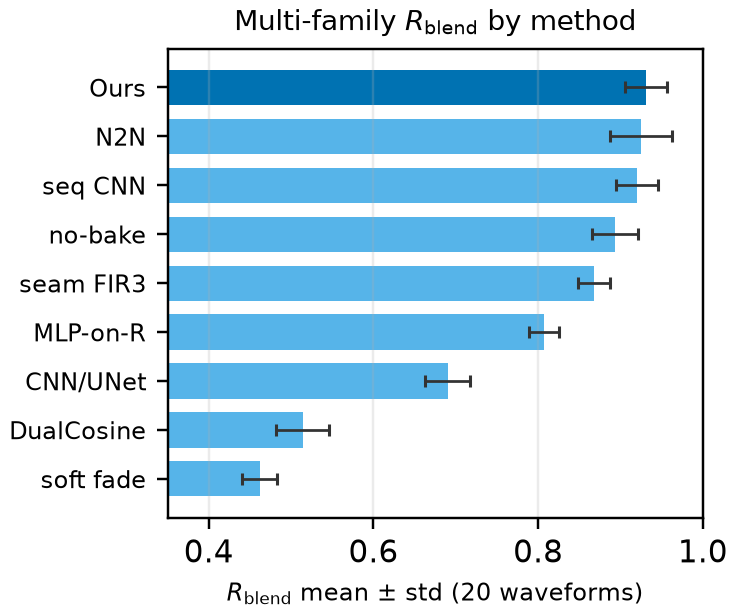
\includegraphics[width=\columnwidth,height=0.42\textheight,keepaspectratio]{figures/fig_sota_method_bars.png}
  \caption{Multi-family mean $R_{\mathrm{blend}}$ by method
  (same $20$-waveform board as Table~\ref{tab:sota-main}).}
  \label{fig:sota-method-bars}
\end{figure}
\FloatBarrier
\clearpage

\begin{figure}[htbp]
  \centering
  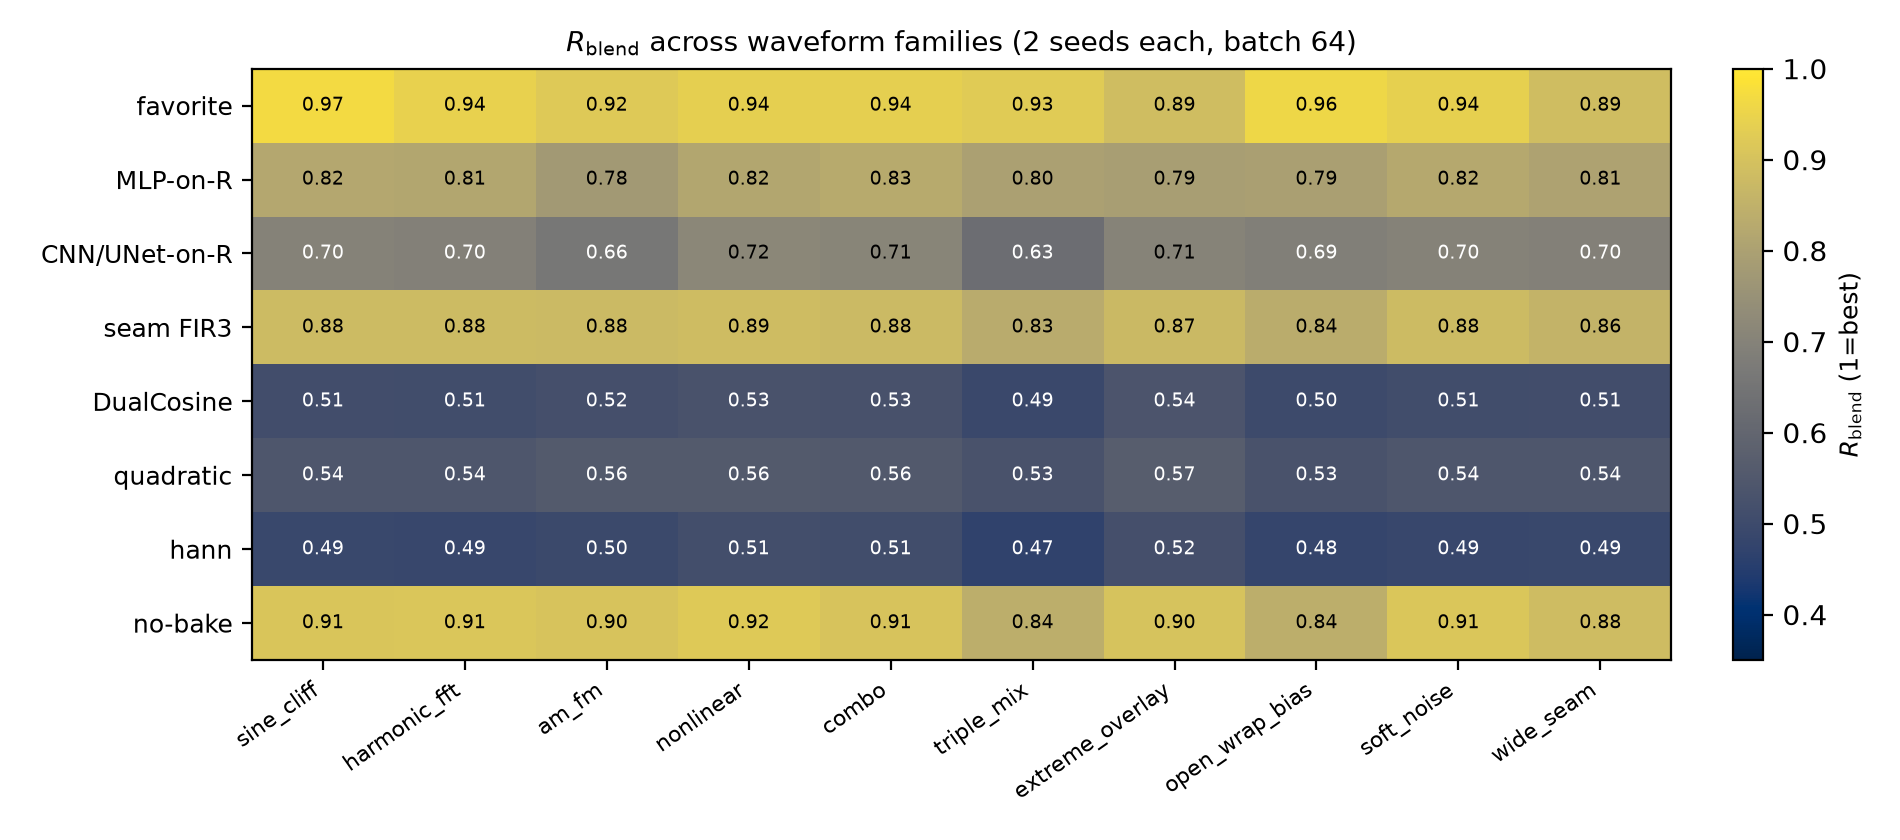
\includegraphics[width=\columnwidth,height=0.42\textheight,keepaspectratio]{figures/fig_sota_heatmap.png}
  \caption{Colorblind-safe (\texttt{cividis}) heatmap of mean $R_{\mathrm{blend}}$
  for selected methods $\times$ generative families (2 seeds each). Higher is better.}
  \label{fig:sota-heatmap}
\end{figure}
\FloatBarrier


\subsection{Multi-family and cliff boards}
\label{sec:app-sota-cliff-tables}

Full multi-family ranking (Table~\ref{tab:sota-main}) and hard-cliff strata
(Table~\ref{tab:cliff-strata}) for the Results narrative in
Sections~\ref{sec:sota-main}--\ref{sec:cliff-strata}.

\begin{table}[htbp]
  \centering
  \caption{Multi-family board (20 waveforms) under $R_{\mathrm{blend}}$ ($\alpha{=}0.7$).
  Core rank columns; SNR/SDR/jump in Table~\ref{tab:sota-main-metrics}.
  $\Delta R$ and ms vs Dual Cosine. N2N/seq seeds \texttt{424242}/\texttt{424243}.}
  \label{tab:sota-main}
  \setlength{\tabcolsep}{3pt}
  \footnotesize
  \begin{tabular}{@{}lrrr@{}}
    \toprule
    Method & $R_{\mathrm{blend}}$ & $\Delta R$ & ms \\
    \midrule
    neural favorite & $0.931\pm0.026$ & ${+}0.417$ & 4.50 \\
    N2N corrupt$\to$corrupt & $0.925\pm0.038$ & ${+}0.410$ & 0.74 \\
    N2N sibling-sup. & $0.924\pm0.035$ & ${+}0.410$ & 0.74 \\
    seq CNN1D & $0.920\pm0.026$ & ${+}0.405$ & 0.53 \\
    no-bake & $0.893\pm0.028$ & ${+}0.379$ & 0.00 \\
    seq LSTM & $0.891\pm0.075$ & ${+}0.376$ & 1.53 \\
    \texttt{seam\_fir3} & $0.868\pm0.019$ & ${+}0.353$ & 0.17 \\
    MLP-on-$R$ & $0.807\pm0.018$ & ${+}0.292$ & 1.76 \\
    CNN/U-Net-on-$R$ & $0.690\pm0.027$ & ${+}0.175$ & 3.08 \\
    DualCosine & $0.514\pm0.032$ & $0$ & 0.98 \\
    soft wide fade & $0.462\pm0.021$ & ${-}0.053$ & 1.87 \\
    \bottomrule
  \end{tabular}
\end{table}
\FloatBarrier

\begin{table}[htbp]
  \centering
  \caption{Multi-family secondary metrics (same board as Table~\ref{tab:sota-main}).}
  \label{tab:sota-main-metrics}
  \setlength{\tabcolsep}{3pt}
  \footnotesize
  \begin{tabular}{@{}lrrr@{}}
    \toprule
    Method & SNR (dB) & SDR (dB) & wrap-jump \\
    \midrule
    neural favorite & $34.6\pm3.2$ & $34.7\pm3.2$ & $0.89\pm0.14$ \\
    N2N corrupt$\to$corrupt & $33.8\pm4.0$ & $33.9\pm4.0$ & $0.89\pm0.15$ \\
    N2N sibling-sup. & $33.9\pm4.1$ & $34.0\pm4.1$ & $0.91\pm0.15$ \\
    seq CNN1D & $32.2\pm3.5$ & $32.4\pm3.5$ & $0.92\pm0.15$ \\
    no-bake & $30.9\pm1.9$ & $31.0\pm1.9$ & $0.91\pm0.15$ \\
    seq LSTM & $32.2\pm5.8$ & $32.4\pm5.8$ & $0.86\pm0.15$ \\
    \texttt{seam\_fir3} & $28.1\pm1.2$ & $28.1\pm1.2$ & $0.46\pm0.08$ \\
    DualCosine & $16.9\pm1.2$ & $16.8\pm1.2$ & $0.32\pm0.05$ \\
    \bottomrule
  \end{tabular}
\end{table}
\FloatBarrier




\begin{table}[htbp]
  \centering
  \caption{Cliff strata on $4{,}096$ holdout tiles under $R_{\mathrm{blend}}$ ($\alpha{=}0.7$).
  Strata by engine wrap-jump ($n$: all $4096$, top25 $1024$, top10 $410$).
  $\pm$ is tile std on the all stratum.}
  \label{tab:cliff-strata}
  \setlength{\tabcolsep}{3pt}
  \footnotesize
  \begin{tabular}{@{}lccc@{}}
    \toprule
    Method & all & top25\% & top10\% \\
    \midrule
    seq LSTM & $0.986\pm0.009$ & 0.989 & 0.990 \\
    N2N sibling-sup. & $0.981\pm0.013$ & 0.985 & 0.985 \\
    N2N corrupt$\to$corrupt & $0.976\pm0.015$ & 0.981 & 0.983 \\
    neural favorite & $0.971\pm0.020$ & 0.978 & 0.978 \\
    seq CNN1D & $0.960\pm0.028$ & 0.969 & 0.970 \\
    no-bake & $0.913\pm0.077$ & 0.929 & 0.922 \\
    \texttt{seam\_fir3} & $0.886\pm0.067$ & 0.870 & 0.869 \\
    DualCosine & $0.525\pm0.239$ & 0.318 & 0.305 \\
    \bottomrule
  \end{tabular}
\end{table}
\FloatBarrier






\subsection{Transfer wrap-protocol status notes}
\label{sec:app-transfer-status}

\begin{table}[htbp]
  \centering
  \caption{Author-method and data-cut status under this wrap-protocol stress test (no invented scores).}
  \label{tab:transfer-sota-status}
  \setlength{\tabcolsep}{3pt}
  \resizebox{\columnwidth}{!}{%
  \begin{adjustbox}{max width=\columnwidth}
\begin{tabular}{@{}lp{0.52\columnwidth}@{}}
    \toprule
    Scope & Note \\
    \midrule
    SeamN2N (ours, N2N-style) & Scored on all seven Table~\ref{tab:transfer-main} boards
      under $R_{\mathrm{blend}}$. Not Lehtinen code \\
    Cycle-GAN (ECG, author) & OOD wrap probe in Table~\ref{tab:transfer-main}
      (MIT-BIH $0.1063$, PTB-XL $0.2105$). Clinical restore $\neq$ wrap residual \\
    BeatDiff (Bedin NeurIPS\,2024) & OOD wrap probe in Table~\ref{tab:transfer-main}
      (MIT-BIH $0.4907$, PTB-XL $0.4933$). Drive prior (not HF).
      Clinical morph prior $\neq$ wrap residual \\
    Paderborn KAt deep (Al~Firdausi CNN) & Trained CNN\_1D\_2L from scratch (not frozen
      \texttt{model.pth}) on bearings K001/KA04/KI04/KB23. File-holdout seed \texttt{20260726},
      train seed \texttt{42}, $20$ epochs. 4-class holdout acc $0.8590$ ($n{=}2560$ segs,
      NORMAL/IR/OR/OR+IR). Classifier wrap residual N/A. Arch-reuse wrap bake listed
      in Table~\ref{tab:transfer-main}$^\dagger$.
      Wrap board: Ours $0.9369$ / SeamN2N $0.8421$ / DualCosine $0.4710$ \\
    Expanded PTB-XL & records500 lead-I expanded ($\sim$2k\,$+$\,\texttt{\_hr} records, board $n{=}256$,
      Ours $0.9451$). Multi-lead still out of scope \\
    Real KIT CNC / IEEE PMU & Synthetic pilots only (download walls) \\
    Formal MOS / MUSHRA & Not collected \\
    \bottomrule
  \end{tabular}
\end{adjustbox}%
  }
\end{table}
\FloatBarrier

\subsection{Matched-budget outer-loop comparison}
\label{sec:meta-approaches-results}

Under a $5{,}000$ evaluation budget with LSTM and xLSTM in the searchable bake vocabulary, Table~\ref{tab:meta-approaches} compares Random NAS, Cont.\ CMA-ES, Arch REINFORCE, Aging evolution, TPE Bayes NAS, and our hybrid GA+PPO approach (Ours). The table reports results from a matched Deferred D1 re-search under locked $R_{\mathrm{blend}}{+}J$ (mean $\pm$ std over three search seeds; artifacts \texttt{meta\_approach\_compare\_v13\_rblend/}). Our hybrid GA+PPO leads with an $R_{\mathrm{blend}}$ of $0.9748{\pm}0.0018$, taking approximately 8.4 hours on average. Aging evolution ranks second at $0.9635{\pm}0.0049$, while Arch REINFORCE shows the highest variance with $0.9599{\pm}0.0116$. Only seed \texttt{1902771841} of our hybrid approach clears the frozen Noise2Noise gate under the short-FitCell D1 protocol, achieving an $R_{\mathrm{blend}}$ of approximately 0.9766 compared to the gate's approximate value of 0.9750. Despite mid-search graphs ranging from about 15k to 370k parameters, our hybrid approach maintains compact models (${\approx}24$k$\pm$2k params across seeds). Since our hybrid method dominated this matched bake-off, the subsequent campaign focuses solely on running hybrid-only FitCell-to-convergence (Section~\ref{sec:v14-converge}, Table~\ref{tab:v14-hybrid-converge}). Note that Noise2Noise is not an outer-loop method in this context (see Tables~\ref{tab:n2n-vs-ours} and~\ref{tab:sota-main}). Learning-curve and bar figures use trajectories from seed \texttt{1902771841} under the same locked objective.

\begin{table}[htbp]
  \centering
  \caption{Matched $5{,}000$-evaluation outer-loop comparison under locked $R_{\mathrm{blend}}{+}J$ (Deferred D1 complete).
    Mean$\pm$std over three search seeds (\texttt{1902771841}, \texttt{2026072701}, \texttt{2026072702}).
    $\Delta R$ uses seed-\texttt{1902771841} Dual Cosine (${\approx}0.504$). Wall-h is mean CUDA wall per approach.
    LSTM?/xLSTM?: whether any seed's champion included that block.}
  \label{tab:meta-approaches}
  \setlength{\tabcolsep}{2pt}
  \scriptsize
  \begin{adjustbox}{max width=\columnwidth}
\begin{tabular}{@{}lrrrcc@{}}
    \toprule
    Method & $R_{\mathrm{blend}}$ & $\Delta R$ vs DC & h & LSTM & xLSTM \\
    \midrule
    Random NAS & $0.9367{\pm}0.0032$ & $+0.4327$ & 4.7 & no & no \\
    Cont.\ CMA-ES & $0.9565{\pm}0.0016$ & $+0.4525$ & 1.8 & no & no \\
    Arch REINFORCE & $0.9599{\pm}0.0116$ & $+0.4559$ & 5.8 & yes & no \\
    Aging evolution & $0.9635{\pm}0.0049$ & $+0.4595$ & 9.0 & yes & no \\
    TPE Bayes NAS & $0.9451{\pm}0.0019$ & $+0.4411$ & 3.8 & no & no \\
    Ours (hybrid GA--PPO) & $0.9748{\pm}0.0018$ & $+0.4708$ & 8.4 & no & no \\
    \bottomrule
  \end{tabular}
\end{adjustbox}
\end{table}


\begin{figure}[htbp]
  \centering
  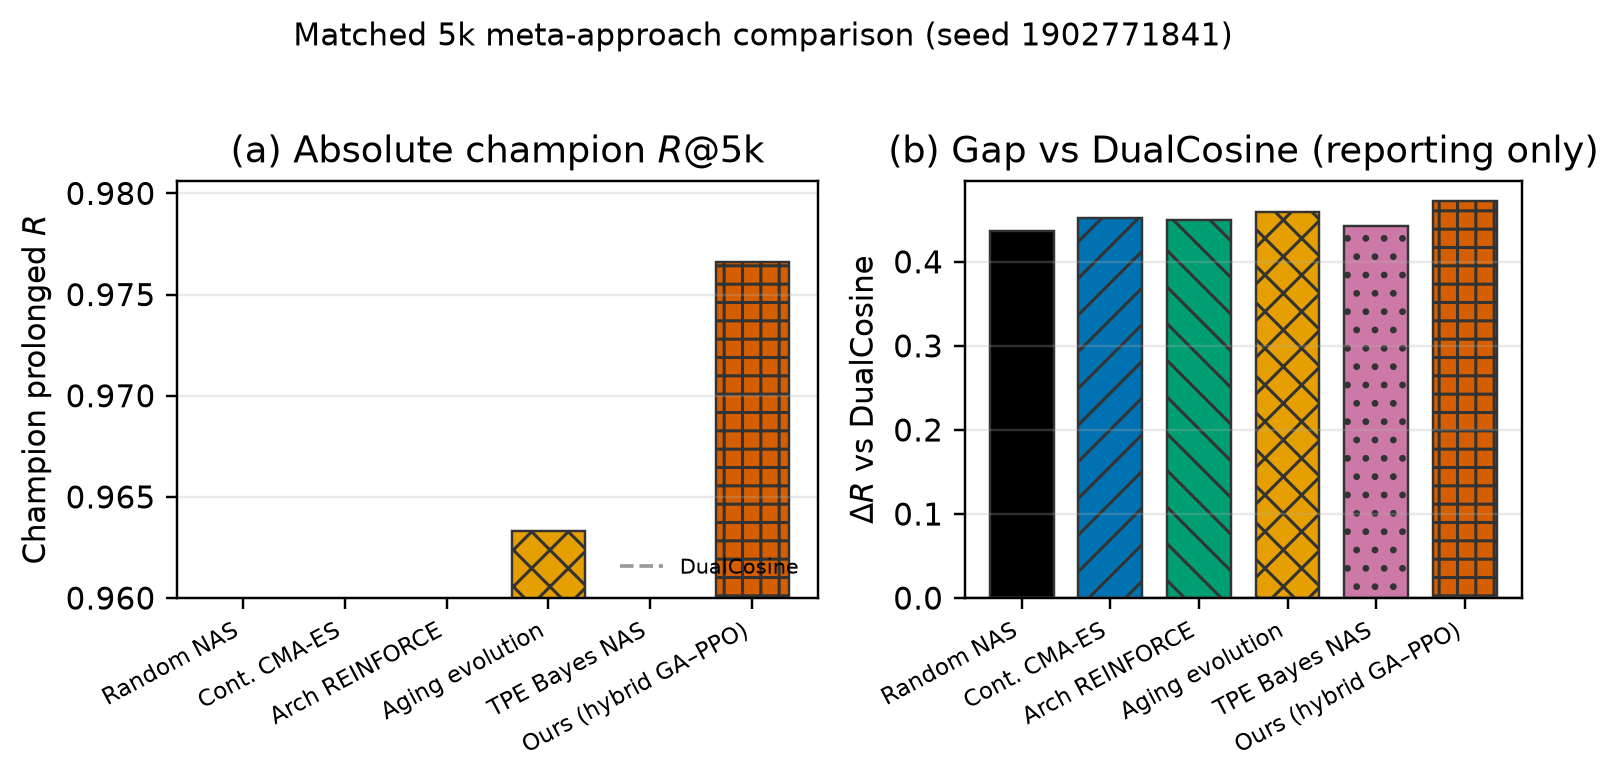
\includegraphics[width=\columnwidth,height=0.42\textheight,keepaspectratio]{figures/meta_approach_bars.png}
  \caption{Matched 5,000-evaluation search methods under locked $R_{\mathrm{blend}}{+}J$ (seed \texttt{1902771841}).
  Table~\ref{tab:meta-approaches} reports mean$\pm$std across three search seeds.
  Dashed line: Dual Cosine on the same runner.}
  \label{fig:meta-approach-bars}
\end{figure}
\FloatBarrier\clearpage

\begin{figure}[htbp]
  \centering
  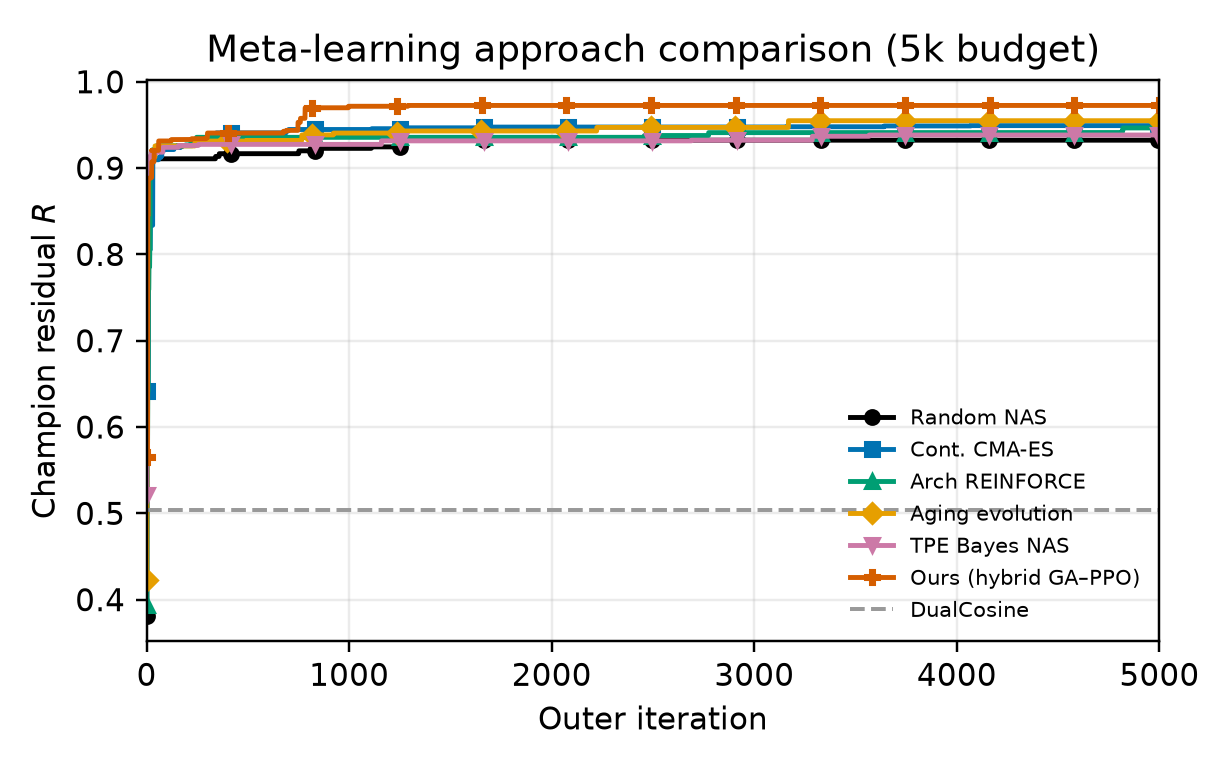
\includegraphics[width=\columnwidth,height=0.42\textheight,keepaspectratio]{figures/fig_meta_approach_compare.png}
  \caption{Champion $R_{\mathrm{blend}}$ over a matched 5,000-evaluation budget (Deferred D1 complete; seed \texttt{1902771841}).
  Dashed line: Dual Cosine.}
  \label{fig:meta-approach-compare}
\end{figure}
\FloatBarrier

\subsection{Ablations and compute}
\label{sec:ablation-compute}

Table~\ref{tab:ablation} answers two narrow questions, not a full factorial re-search of Table~\ref{tab:meta-approaches}.
\textbf{Left column:} within one recorded hybrid history under the superseded prolonged-$R$ search metric, what was the best freeze tagged by outer-loop branch (PPO/GA/PBT/\ldots) at the $5$k gate?
These are branch labels in a single run, not separately fitted champions, so they mainly show that no single branch monopolizes the trajectory.
\textbf{Right column:} isolated $150$-iteration \texttt{ablate-*} restarts (seed \texttt{1902771841}) whose final cells are re-scored under locked $R_{\mathrm{blend}}$.
They probe whether dropping GA or PPO collapses residual under a short budget; they are \emph{not} matched-$5$k competitors and must not overwrite Table~\ref{tab:meta-approaches}.
\paragraph{How to read Table~\ref{tab:ablation}.}
Left-column values are close to each other (${\approx}0.987$--$0.991$ prolonged $R$): in that single history, branch tags do not identify a unique winner, so we do not treat ``GA-only freeze'' as proof that GA alone suffices under locked $R_{\mathrm{blend}}$.
Right-column short restarts under $R_{\mathrm{blend}}$ stay far below the matched-$5$k hybrid mean ($0.9748$) and the converge seed ($0.9912$) because the budget is only $150$ iterations with short FitCell---they are sensitivity checks, not leaderboard rows.
The matched comparison that drives method choice remains Table~\ref{tab:meta-approaches}.
Table~\ref{tab:compute} summarizes campaign compute (historical prolonged-$R$ overnight).

\begin{table}[htbp]
  \centering
  \caption{Ablations (interpret narrowly).
    Left: best prolonged $R$ by branch label in one hybrid history (final iteration ${\approx}6{,}922$; superseded search metric; not separate fits).
    Right: isolated 150-iteration \texttt{ablate-*} final champions re-scored under $R_{\mathrm{blend}}$ ($\alpha{=}0.7$; seed \texttt{1902771841}).
    Full $R_{\mathrm{blend}}$ branch re-search remains deferred; use Table~\ref{tab:meta-approaches} for matched outer-loop comparison.}
  \label{tab:ablation}
  \setlength{\tabcolsep}{3pt}
  \begin{adjustbox}{max width=\columnwidth}
  \begin{tabular}{@{}lrr@{}}
    \toprule
    Config & Prolonged $R$ freeze & 150-it $R_{\mathrm{blend}}$ \\
    \midrule
    Full hybrid & 0.99093 & 0.92710 \\
    GA-only & 0.99016 & 0.94168 \\
    PBT (search branch) & 0.99012 & n/a \\
    PPO-only & 0.98924 & 0.94405 \\
    GA+PPO & n/a & 0.94478 \\
    Combined branch & 0.98854 & n/a \\
    NAS branch & 0.98677 & n/a \\
    Dual Cosine (runner) & 0.81658 & ${\approx}0.539$ \\
    \bottomrule
  \end{tabular}
\end{adjustbox}
\end{table}
\FloatBarrier

\begin{table}[htbp]
  \centering
  \caption{Compute budget for the reported 5,000-evaluation search run (RTX~3090, search seed \texttt{1902771841}; prolonged-$R$ objective).
    Final champion $R$ below is the historical prolonged freeze, not $R_{\mathrm{blend}}$.}
  \label{tab:compute}
  \setlength{\tabcolsep}{3pt}
  \begin{adjustbox}{max width=\columnwidth}
\begin{tabular}{@{}lr@{}}
    \toprule
    Item & Value \\
    \midrule
    GPU & NVIDIA GeForce RTX 3090 \\
    Elapsed wall time & ${\approx}7.92$\,h \\
    Clean iterations / arch evals & ${\approx}6{,}922$ \\
    Population size & 12 \\
    Final champion prolonged $R$ & 0.99093 \\
    Dual Cosine baseline (runner, prolonged) & 0.81658 \\
    Peak VRAM (replay) & ${\approx}3.29$\,GiB \\
    \bottomrule
  \end{tabular}
\end{adjustbox}
\end{table}
\FloatBarrier

\subsection{Hyperparameter sensitivity}
\label{para:hp-sensitivity}
One-at-a-time $\pm 50\%$ probe of Table~\ref{tab:hyperparams} knobs at $500$ outer iterations (seed \texttt{1902771841}).
Not a full $5$k re-search.
Default champion $R{\approx}0.9888$. The largest $|\Delta R|$ among OAT arms is ${\approx}0.0123$ (50\% lower learning rate).
All $11/11$ arms finished under this budget.

% Auto-generated by scripts/bench_meta_hp_sensitivity.py — do not hand-edit.
\begin{table}[htbp]
  \centering
  \small
  \caption{One-at-a-time $\pm 50\%$ hyperparameter sensitivity probe (500 outer iterations, seed \texttt{1902771841}, sine{+}cliff FitCell). Champion absolute $R$ is compared with the Table~\ref{tab:hyperparams} default. This is sensitivity evidence only, not a full 5,000-iteration re-search for each parameter.}
  \label{tab:hp-sensitivity}
  \setlength{\tabcolsep}{3pt}
  \footnotesize
  \begin{adjustbox}{max width=\columnwidth}
\begin{tabular}{@{}lrrr@{}}
    \toprule
    Parameter change & Champ.\ $R$ & $\Delta R$ & Iter. \\
    \midrule
    Default & 0.98882 & +0.00000 & 500 \\
    Population size $-50\%$ & 0.98136 & -0.00746 & 500 \\
    Population size $+50\%$ & 0.98073 & -0.00809 & 500 \\
    PPO clip $-50\%$ & 0.98159 & -0.00723 & 500 \\
    PPO clip $+50\%$ & 0.99041 & +0.00159 & 500 \\
    Learning rate $-50\%$ & 0.97654 & -0.01228 & 500 \\
    Learning rate $+50\%$ & 0.98138 & -0.00744 & 500 \\
    GA mutation rate $-50\%$ & 0.98334 & -0.00548 & 500 \\
    GA mutation rate $+50\%$ & 0.99002 & +0.00120 & 500 \\
    PPO entropy $-50\%$ & 0.98912 & +0.00030 & 500 \\
    PPO entropy $+50\%$ & 0.99116 & +0.00234 & 500 \\
    \bottomrule
  \end{tabular}
\end{adjustbox}
\end{table}


\begin{figure}[htbp]
  \centering
  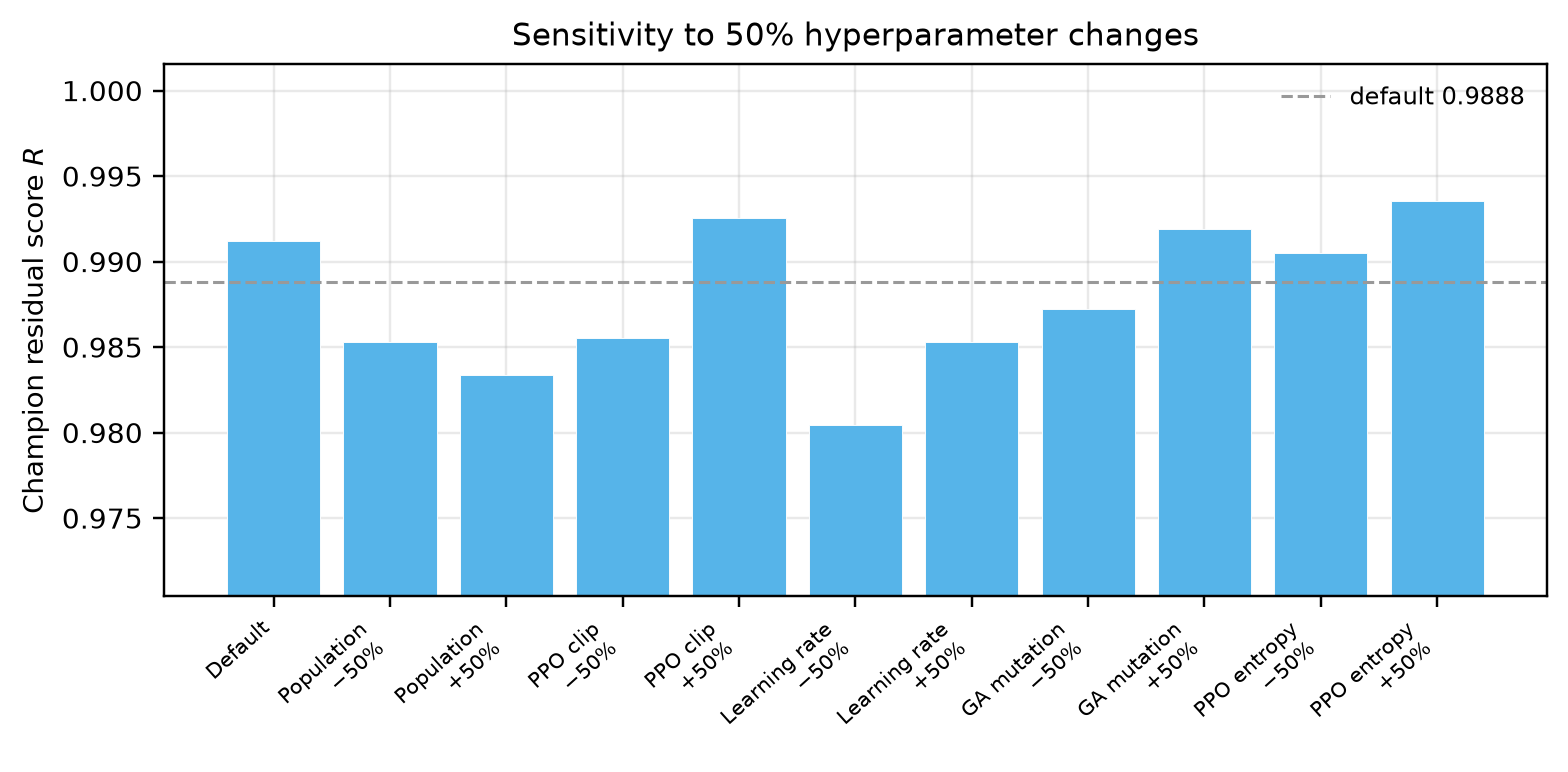
\includegraphics[width=\linewidth,height=0.42\textheight,keepaspectratio]{figures/fig_meta_hp_sensitivity.png}
  \caption{One-at-a-time $\pm 50\%$ HP sensitivity of hybrid champion $R$ at 500 iterations. Blue bar: Table~\ref{tab:hyperparams} default.}
  \label{fig:hp-sensitivity}
\end{figure}
\FloatBarrier

\subsection{Transfer inference latency}
\label{sec:transfer-latency-app}
Table~\ref{tab:transfer-latency} and Figure~\ref{fig:signal-heal-transfer-latency} pair with the prolonged-$R$ transfer board (Table~\ref{tab:transfer-main}).
N2N latency uses the wavetable checkpoint zero-shot. Domain-trained N2N quality scores are in Table~\ref{tab:transfer-main}.

\begin{table}[htbp]
  \centering
  \caption{Transfer-domain inference latency (ms/batch). Batch=64, CUDA.}
  \label{tab:transfer-latency}
  \setlength{\tabcolsep}{4pt}
  \begin{adjustbox}{max width=\columnwidth}
\begin{tabular}{@{}lrrrrrr@{}}
    \toprule
    Method & CWRU & MFPT & MIT-BIH & PTB-XL & CNC & PMU \\
    \midrule
    no-bake & 0.26 & 0.26 & 0.27 & 0.27 & 0.28 & 0.26 \\
    Dual Cosine & 1.10 & 1.11 & 1.12 & 1.14 & 1.15 & 1.14 \\
    Ours (hybrid) & 3.92 & 6.61 & 2.87 & 1.67 & 1.69 & 1.67 \\
    N2N (WT to domain) & 0.95 & 0.99 & 0.98 & 0.97 & 0.98 & 0.97 \\
    \bottomrule
  \end{tabular}
\end{adjustbox}
\end{table}
\FloatBarrier

\begin{figure}[htbp]
  \centering
  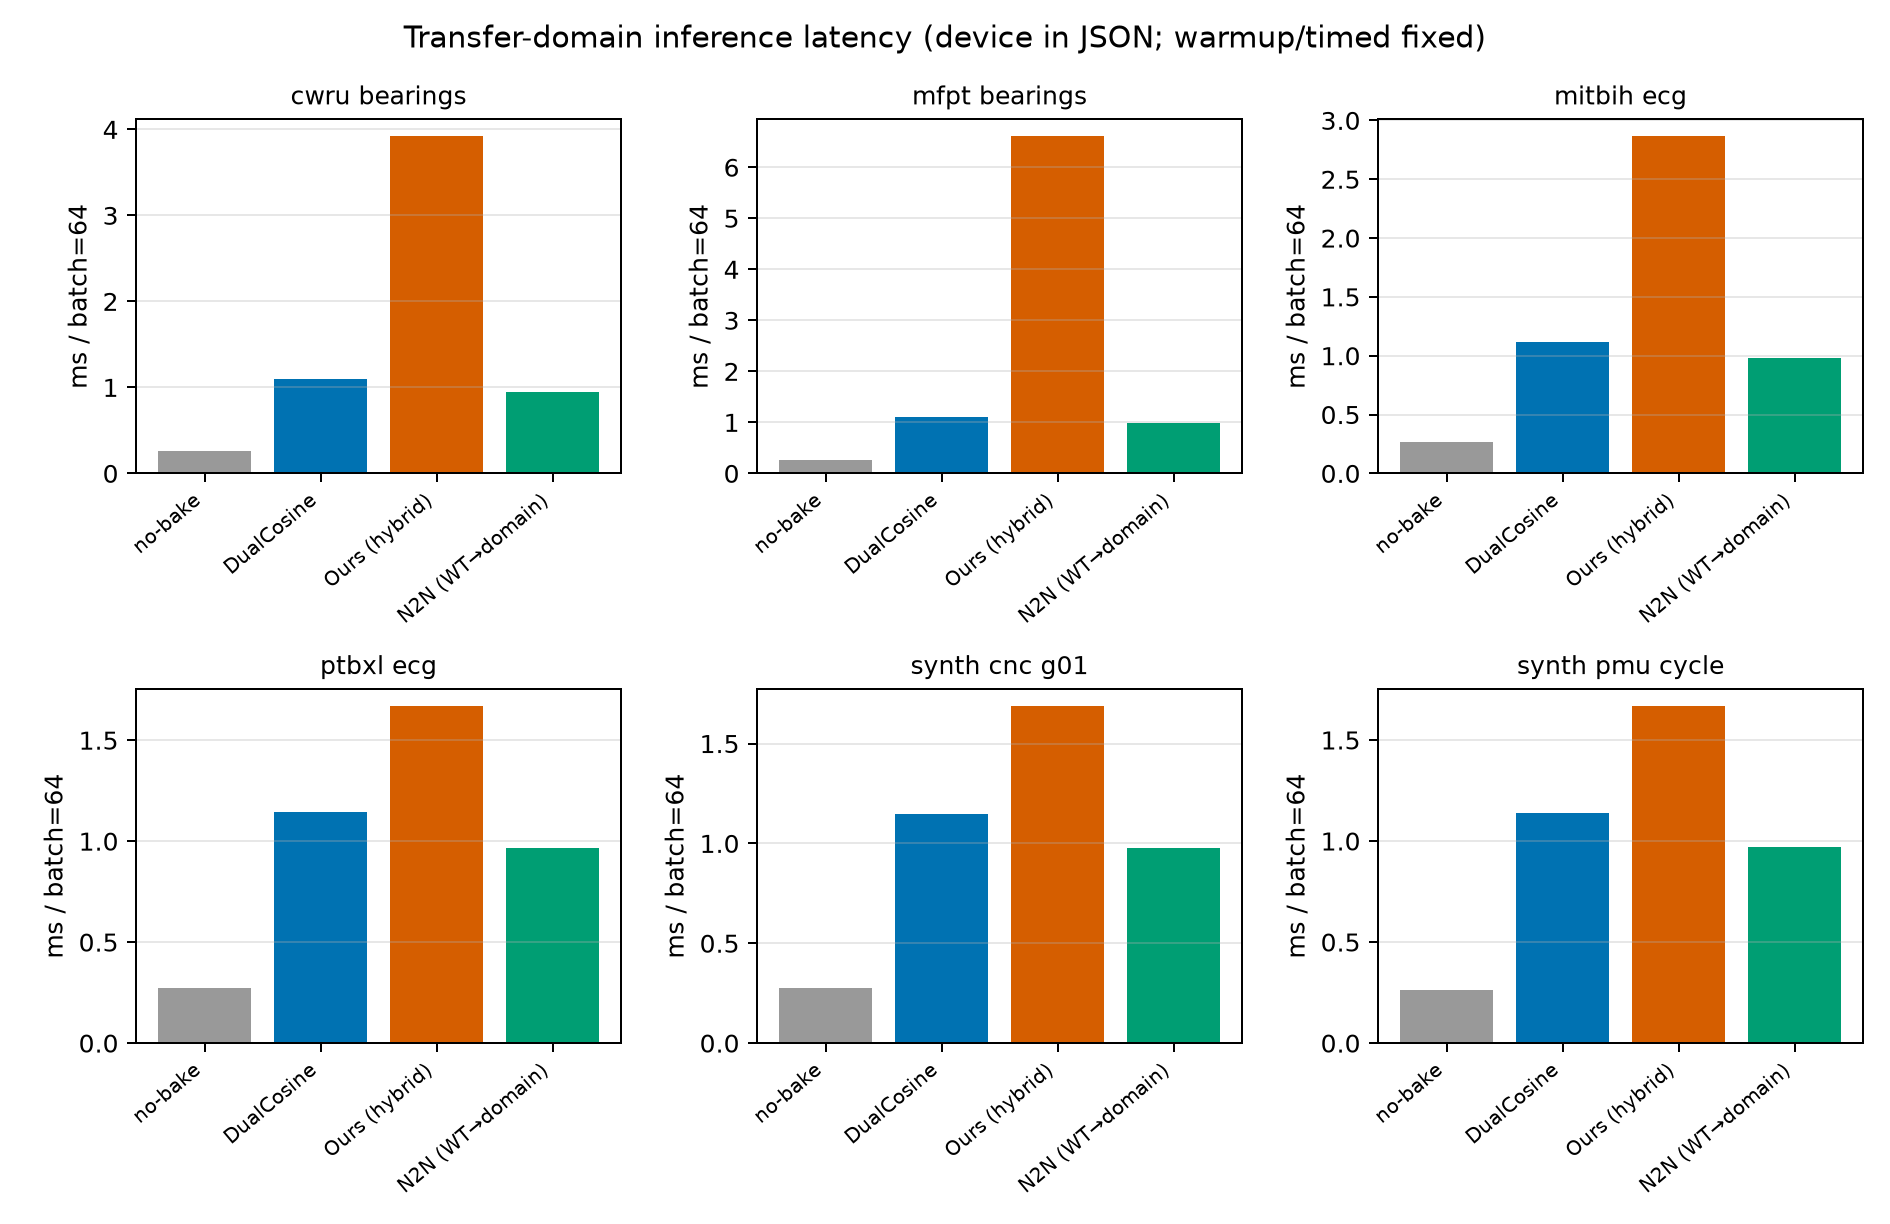
\includegraphics[width=\columnwidth,height=0.42\textheight,keepaspectratio]{figures/fig_signal_heal_transfer_latency.png}
  \caption{Transfer-domain inference latency (ms/batch). N2N is wavetable-trained zero-shot when available.}
  \label{fig:signal-heal-transfer-latency}
\end{figure}
\FloatBarrier

\subsection{Search-monitor figures}
\label{sec:search-monitor-figs}

\begin{figure}[htbp]
  \centering
  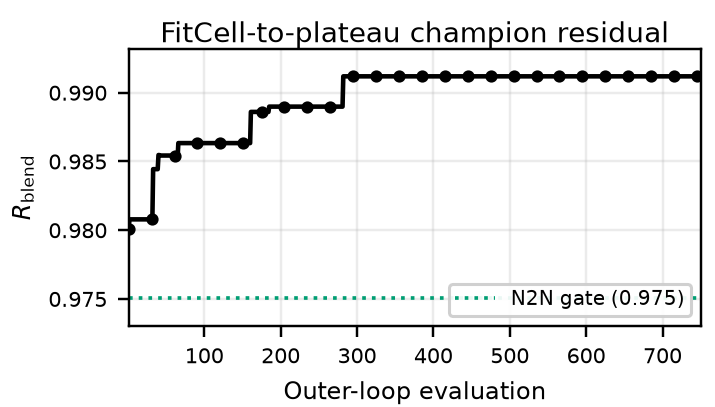
\includegraphics[width=\columnwidth,height=0.42\textheight,keepaspectratio]{figures/champ_residual_vs_iter.png}
  \caption{FitCell-to-plateau champion $R_{\mathrm{blend}}$ vs.\ outer-loop evaluation
  (seed \texttt{1902771841}; y-axis zoomed to the high-$R$ regime with Noise2Noise gate marked).}
  \label{fig:champ-residual}
\end{figure}
\FloatBarrier

\begin{figure}[htbp]
  \centering
  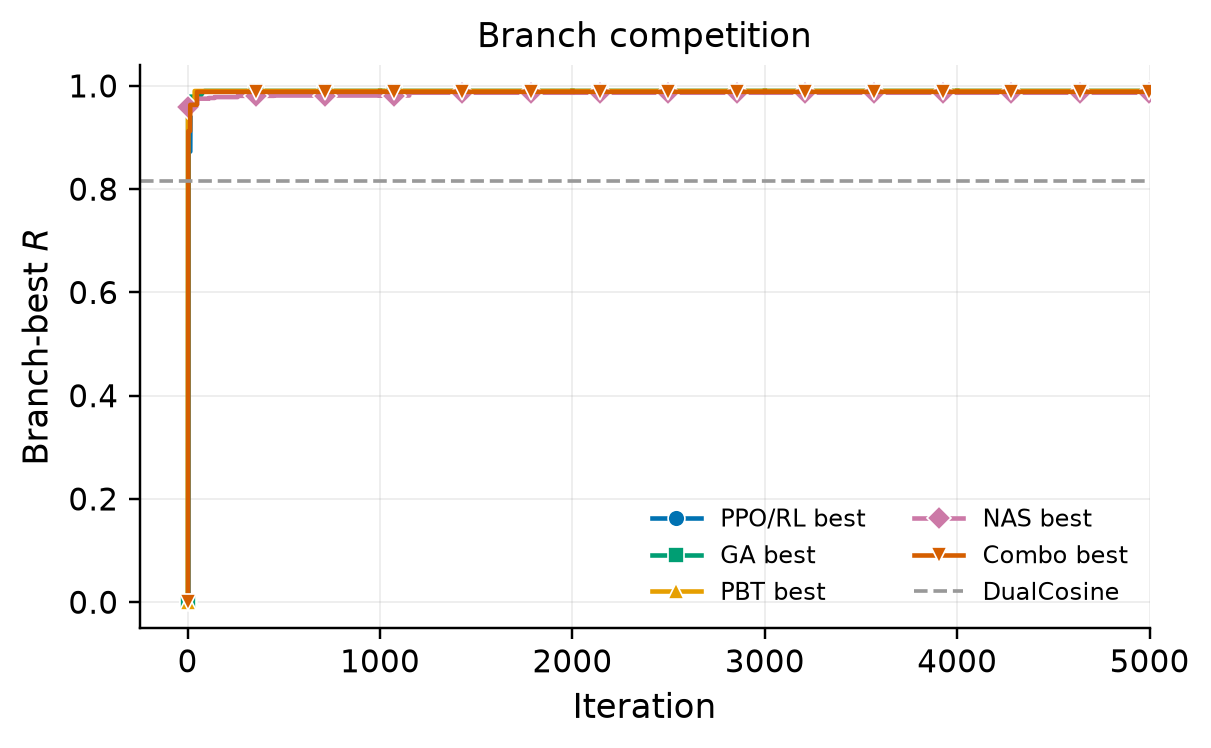
\includegraphics[width=\columnwidth,height=0.42\textheight,keepaspectratio]{figures/branch_bests_vs_iter.png}
  \caption{Best residual by search branch (older overnight monitor freeze; search-trace artifact).}
  \label{fig:branch-bests}
\end{figure}
\FloatBarrier

\begin{figure}[htbp]
  \centering
  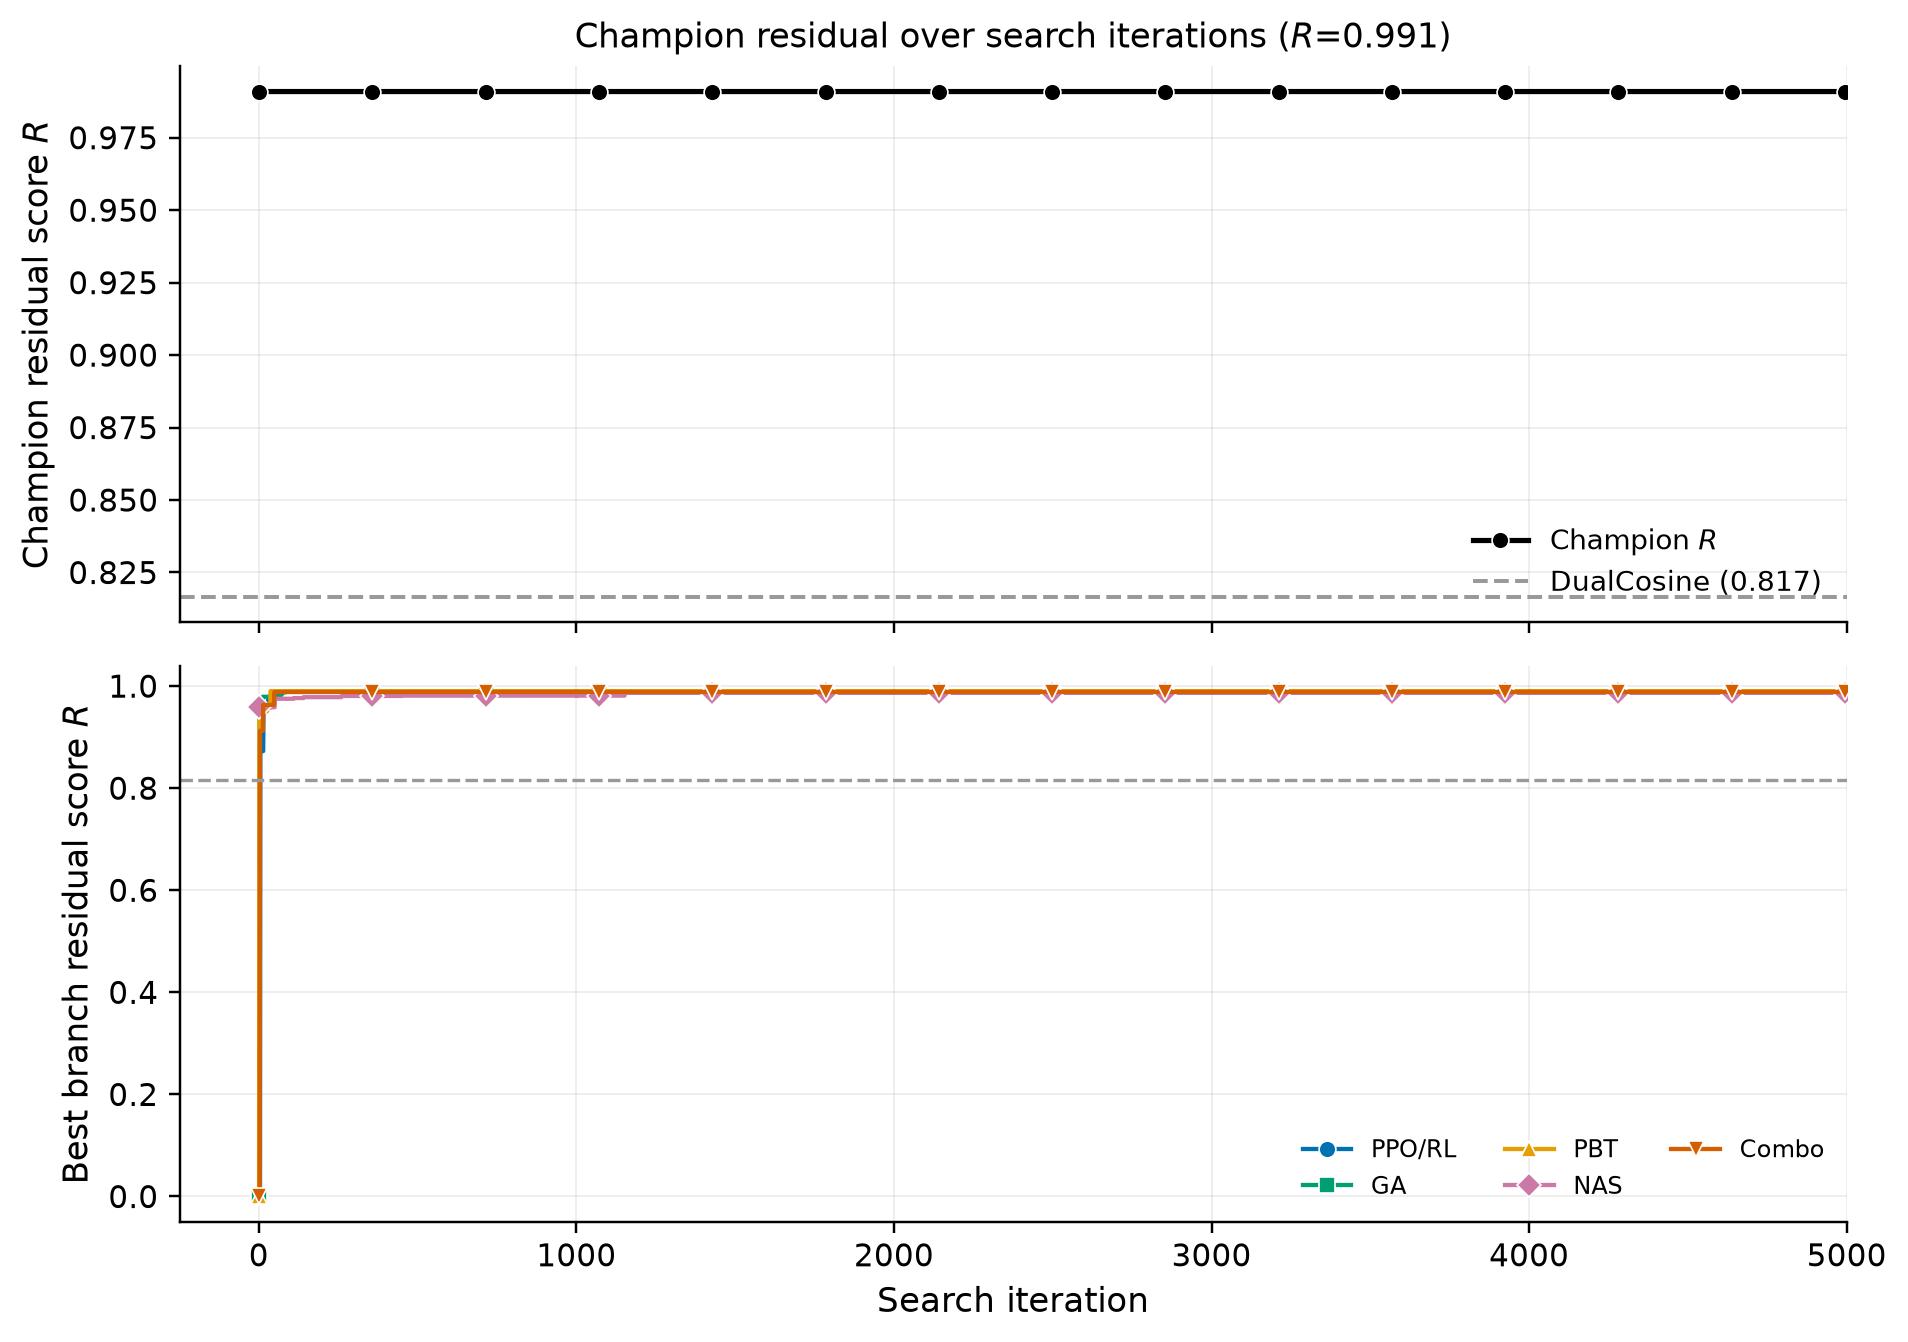
\includegraphics[width=\columnwidth,height=0.42\textheight,keepaspectratio]{figures/search_panel.png}
  \caption{Search progress: champion $R$ (top) and branch bests (bottom).}
  \label{fig:search-panel}
\end{figure}
\FloatBarrier

\begin{figure}[htbp]
  \centering
  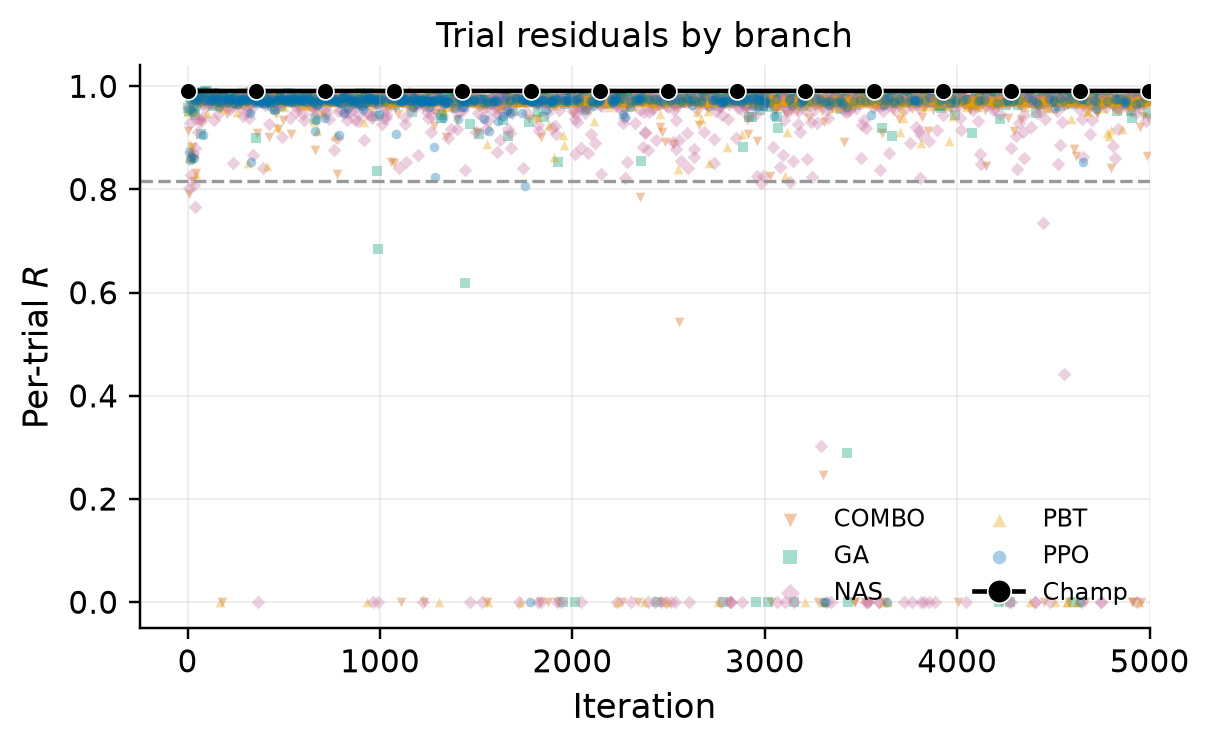
\includegraphics[width=\columnwidth,height=0.42\textheight,keepaspectratio]{figures/residual_by_branch.png}
  \caption{Per-trial residual by branch with champion trajectory overlaid.}
  \label{fig:residual-branch}
\end{figure}
\FloatBarrier

\begin{figure}[htbp]
  \centering
  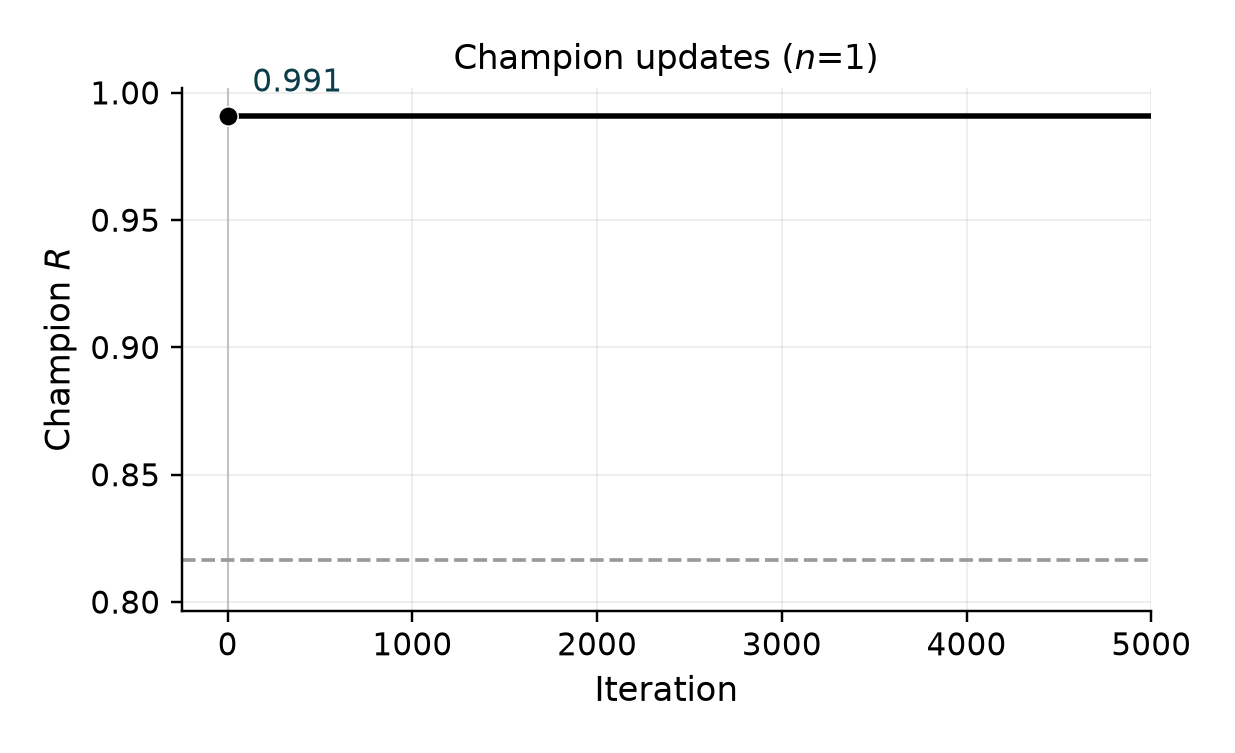
\includegraphics[width=\columnwidth,height=0.42\textheight,keepaspectratio]{figures/champion_timeline.png}
  \caption{Champion updates (older overnight monitor freeze; search-trace artifact).}
  \label{fig:champ-timeline}
\end{figure}
\FloatBarrier

\subsection{Inference and classical diagnostic plots}
\label{sec:app-inference-diags}

\begin{figure}[htbp]
  \centering
  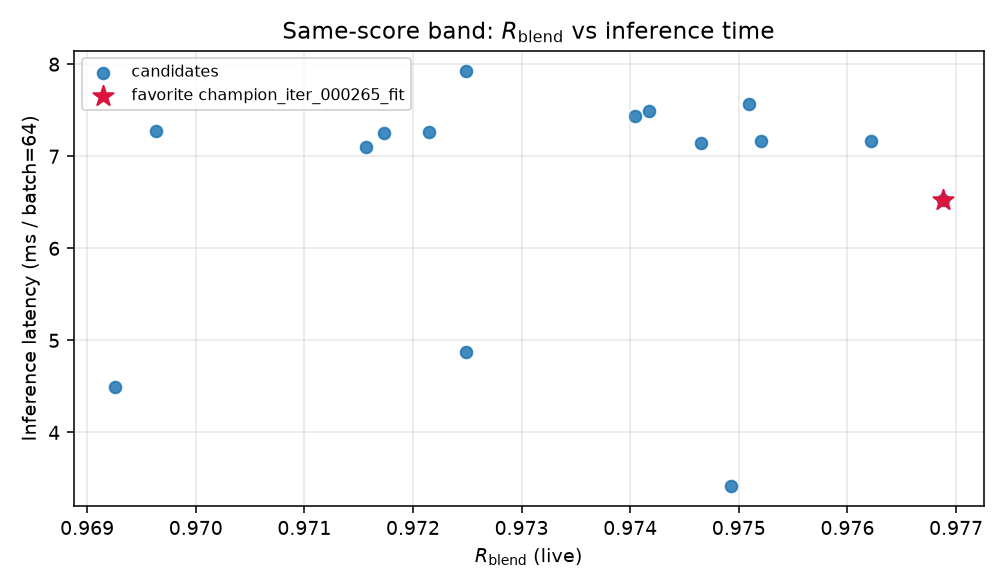
\includegraphics[width=\columnwidth,height=0.42\textheight,keepaspectratio]{figures/fig_inference_vs_residual.png}
  \caption{High-$R$ fitted operators: residual vs CUDA latency. Star: favorite.}
  \label{fig:inference-pareto}
\end{figure}
\FloatBarrier

\begin{figure}[htbp]
  \centering
  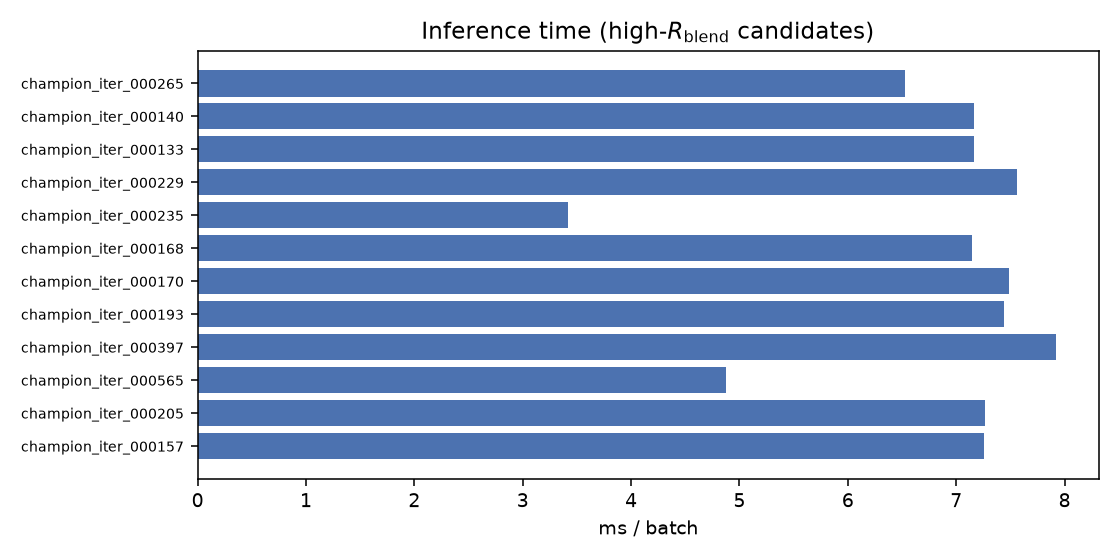
\includegraphics[width=\columnwidth,height=0.42\textheight,keepaspectratio]{figures/fig_inference_latency_bars.png}
  \caption{Inference latency for high-$R$ fitted models (CUDA, batch 64).}
  \label{fig:inference-bars}
\end{figure}
\FloatBarrier

\begin{figure}[htbp]
  \centering
  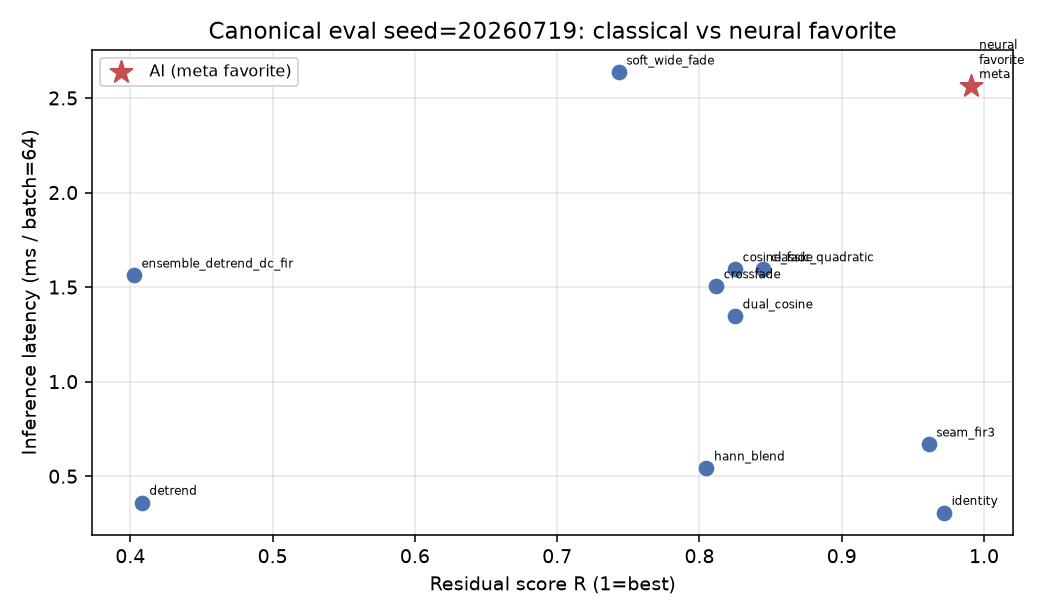
\includegraphics[width=\columnwidth,height=0.42\textheight,keepaspectratio]{figures/fig_classical_vs_ai_scatter.png}
  \caption{Canonical holdout: classical methods and favorite in the $R$ vs ms/batch plane.}
  \label{fig:classical-vs-ai-scatter}
\end{figure}
\FloatBarrier

\begin{figure}[htbp]
  \centering
  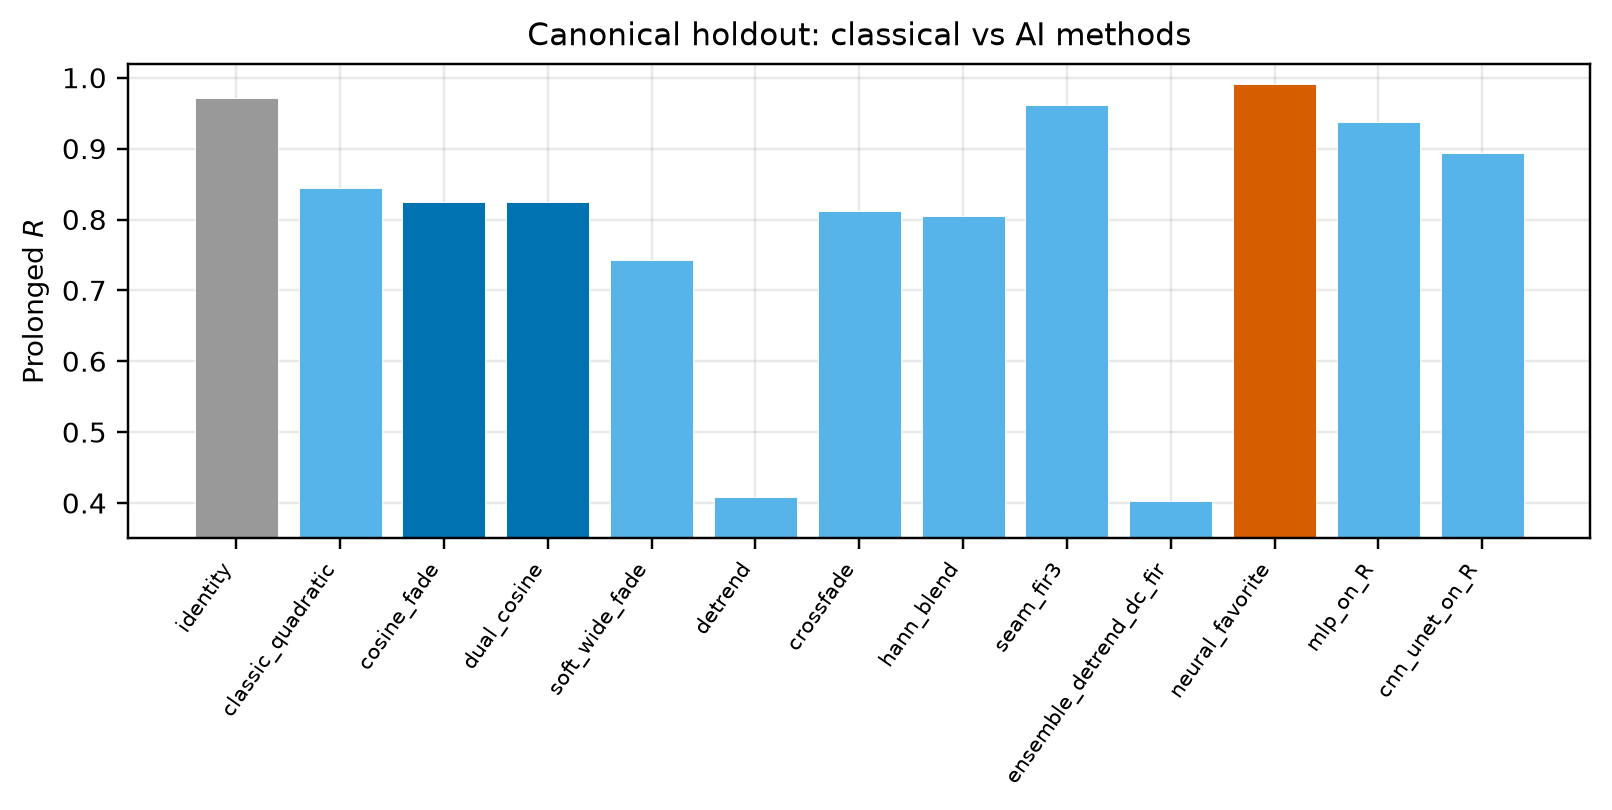
\includegraphics[width=\columnwidth,height=0.42\textheight,keepaspectratio]{figures/fig_classical_vs_ai_bars.png}
  \caption{Canonical holdout ranking on $R_{\mathrm{blend}}$ (left) and latency (right).}
  \label{fig:classical-vs-ai-bars}
\end{figure}
\FloatBarrier
